\documentclass[11pt]{article}

\usepackage[margin=1in]{geometry}
\usepackage{amsmath,amssymb,amsthm}
\usepackage{booktabs}
\usepackage{graphicx}
\usepackage{xcolor}
\usepackage{microtype}
\usepackage{hyperref}
\usepackage{url}

\hypersetup{
  colorlinks=true,
  linkcolor=blue!55!black,
  citecolor=blue!55!black,
  urlcolor=blue!55!black,
  pdftitle={A computer-assisted proof of an unequal-mass Moth-I 13 periodic orbit},
  pdfauthor={Rexyysilent}
}

\newtheorem{theorem}{Theorem}
\newtheorem{corollary}[theorem]{Corollary}
\newtheorem{lemma}[theorem]{Lemma}
\newtheorem{remark}[theorem]{Remark}
\newcommand{\R}{\mathbb{R}}
\newcommand{\PhiFlow}{\Phi}
\newcommand{\cross}{\mathbin{\times}}

\title{A computer-assisted proof of an unequal-mass\\
Moth-I$^{13}$ periodic orbit in the planar Newtonian three-body problem}
\author{Rexyysilent}
\date{August 2026}

\begin{document}
\maketitle

\begin{abstract}
We give a computer-assisted proof of a collisionless periodic solution of the planar Newtonian three-body problem with exact masses
$(m_1,m_2,m_3)=(1,1,1001/1000)$ and zero angular momentum. In a fixed Euler normalization, the two unit masses start at $(-1,0)$ and $(1,0)$, the third mass starts at the origin, and the initial velocity is enclosed in an explicit interval box. Reversing symmetry reduces periodicity to a half-return problem. A 244-segment multiple-shooting formulation gives a 1,955-dimensional zero problem, which is validated by outward-rounded Taylor/Picard integration and a strict Krawczyk inclusion. A full-time interval tube proves that every squared pair distance is greater than $0.003$. Numerically, the solution has period about $193.9144360215894$, syzygy word $(2132123123123213)^{13}$, and the geometry of a Moth-I$^{13}$ satellite. A finite audit of the principal public catalogs found no equivalent orbit at this exact rational mass triple. Accordingly, the catalog claim is only that this realization is apparently uncatalogued; neither a new topological class nor unconditional priority is claimed. Minimal-period primitivity and the displayed syzygy word remain numerical characterizations rather than parts of the interval theorem.
\end{abstract}

\section{Introduction}

The planar Newtonian three-body problem has a long history of numerical discoveries, from the figure-eight choreography to large modern catalogs of collisionless periodic solutions. Computer-assisted proofs are needed when the desired conclusion is existence of an exact orbit rather than the observation of a small floating-point return residual. Earlier rigorous work established choreographies by interval Newton and Krawczyk methods \cite{kapela-zgliczynski-2003}. Kapela and Sim\'o developed the multiple-shooting and first-integral framework that is the closest direct precedent for the present calculation \cite{kapela-simo-2007}; the CAPD ecosystem provides a general rigorous ordinary-differential-equation framework for such arguments \cite{capd-2020}.

This paper validates one unequal-mass, zero-angular-momentum solution suggested by continuation from a known equal-mass Moth-I satellite. The result is stated in a normalization that removes translation, rotation, and Newtonian scaling. Its proof combines four ingredients:
\begin{enumerate}
  \item an exact reversing symmetry that converts a half-return into a periodic orbit;
  \item a square 1,955-dimensional multiple-shooting system;
  \item outward-rounded enclosures of the flow, its first derivative, and the Krawczyk operator; and
  \item a positive interval lower bound for all three pair distances on the full orbit.
\end{enumerate}

The distinctions among proof, numerical characterization, and catalog audit are important. The interval theorem proves existence, collisionlessness, and local uniqueness in the certified shooting box. It does not prove that the displayed period is minimal. The topology is a proper power, so the symbolic word alone cannot distinguish a primitive satellite from repeated traversal of a shorter orbit. The word and primitivity are therefore reported as numerical evidence. Finally, failure to find a match in finite public catalogs supports an ``apparently uncatalogued'' claim but cannot establish universal priority.

General existence theorems do not replace this computation. In particular, the theorem realizing reduced syzygy classes for near-equal masses concerns sufficiently small nonzero angular momentum and relative periodicity; it does not certify this exact zero-angular-momentum, inertially closed solution \cite{moeckel-montgomery-2015}.

\section{Newtonian model and normalization}

Let $q_i,v_i\in\R^2$ and let $m_1=m_2=1$, $m_3=\mu=1001/1000$. With gravitational constant $G=1$, the equations are
\begin{equation}
  \dot q_i=v_i,\qquad
  \dot v_i=\sum_{j\ne i}m_j\frac{q_j-q_i}{\lVert q_j-q_i\rVert^3},
  \qquad i=1,2,3. \label{eq:newton}
\end{equation}
They are analytic away from binary collisions and preserve total momentum, center of mass, energy, and scalar angular momentum
\begin{equation}
  L=\sum_{i=1}^3m_i\,q_i\cross v_i . \label{eq:angular}
\end{equation}

The initial configuration is fixed as
\begin{equation}
  q_1(0)=(-1,0),\qquad q_2(0)=(1,0),\qquad q_3(0)=(0,0), \label{eq:q0}
\end{equation}
with velocities
\begin{equation}
  v_1(0)=v_2(0)=(a,b),\qquad
  v_3(0)=-\frac{2}{\mu}(a,b). \label{eq:v0}
\end{equation}
Thus center of mass, total momentum, and angular momentum vanish exactly. The position normalization fixes translation, rotation, and Newtonian scale; the reversing section below fixes phase.

The certified parameter box is centered at
\begin{align}
  \bar a={}&0.4632255424493246161961696989282234060071831741469930094981680221404365091354,\\
  \bar b={}&0.3988159832923292289438092857690976537647786038697180258349617695394316511243,\\
  \bar\tau={}&96.95721801079469532830593565994101358608358855157701178127825277217753836265,
\end{align}
with radii $10^{-14}$, $10^{-14}$, and $10^{-13}$ respectively. Here $\tau$ is the half-period.

\section{Reversing symmetry and the half-return theorem}

Let $P_{12}$ exchange the two unit-mass labels. Define
\begin{equation}
  \mathcal R(q_1,q_2,q_3;v_1,v_2,v_3)
  =(-q_2,-q_1,-q_3;v_2,v_1,v_3). \label{eq:reverser}
\end{equation}
The spatial half-turn followed by $P_{12}$ is an ordinary symmetry of \eqref{eq:newton}; composing it with velocity reversal gives \eqref{eq:reverser}. Consequently
\begin{equation}
  \mathcal R^2=I,\qquad \mathcal R\PhiFlow_t=\PhiFlow_{-t}\mathcal R. \label{eq:reversing}
\end{equation}
The initial state \eqref{eq:q0}--\eqref{eq:v0} lies in $\operatorname{Fix}(\mathcal R)$.

We reduce translation and total momentum by retaining
$x=(q_1,q_2,v_1,v_2)\in\R^8$ and setting
\begin{equation}
  q_3=-\frac{q_1+q_2}{\mu},\qquad
  v_3=-\frac{v_1+v_2}{\mu}. \label{eq:com-reduction}
\end{equation}
At time $\tau$, define the boundary function
\begin{equation}
  B(x)=\left(q_{1x}+q_{2x},\ q_{1y}+q_{2y},\ q_1\mathbin{\cdot}(v_1-v_2)\right). \label{eq:boundary}
\end{equation}

\begin{lemma}[Half-return closure]\label{lem:closure}
The collisionless solution from \eqref{eq:q0}--\eqref{eq:v0} is $2\tau$-periodic whenever $B(x(\tau))=0$.
\end{lemma}

\begin{proof}
The first two components of $B=0$, together with \eqref{eq:com-reduction}, imply $q_2=-q_1$ and $q_3=0$ at time $\tau$. Conservation of the initially zero angular momentum gives
\[
  0=L=q_1\cross(v_1-v_2).
\]
The third component of $B=0$ gives $q_1\cdot(v_1-v_2)=0$. Collisionlessness implies $q_1\ne0$, hence $v_1=v_2$. Total momentum then gives $v_3=-2v_1/\mu$, so $x(\tau)\in\operatorname{Fix}(\mathcal R)$. Two intersections with the fixed set of a reversing involution imply
$\PhiFlow_{2\tau}(x(0))=x(0)$ by \eqref{eq:reversing}.
\end{proof}

\section{Multiple shooting and the Krawczyk problem}

Put $N=244$ and $h=\tau/N$. Let $X_0=\iota(a,b)$ be the reduced initial state defined by \eqref{eq:q0}--\eqref{eq:v0}; the unknowns are
\begin{equation}
  z=(a,b,\tau,X_1,\ldots,X_N)\in\R^{3+8N}=\R^{1955}. \label{eq:unknowns}
\end{equation}
For the reduced flow $\phi_h$, define
\begin{align}
  G_i(z)&=X_i-\phi_h(X_{i-1}), && i=1,\ldots,N,\\
  G_{N+1}(z)&=B(X_N). \label{eq:shooting}
\end{align}
This is a square system of $8N+3$ equations. Segmenting the long, unstable half-orbit prevents the wrapping that would make a single interval propagation unusable.

For an interval box $Z$ centered at $\bar z$, let $[DG(Z)]$ enclose every Jacobian of $G$ on $Z$, and let $C$ be the stored point preconditioner. The verified Krawczyk set is
\begin{equation}
  K(Z)=\bar z-CG(\bar z)+\bigl(I-C[DG(Z)]\bigr)(Z-\bar z). \label{eq:krawczyk}
\end{equation}
All arithmetic used to bound \eqref{eq:krawczyk} is outward rounded. The implementation exploits the block-bidiagonal shooting structure; the finite stored preconditioner is not assumed to be an exact inverse, and its defect $I-CA_0$ is included explicitly \cite{krawczyk-1969}.

\begin{theorem}[Certified periodic orbit]\label{thm:main}
For the exact masses $(1,1,1001/1000)$, there exists a collisionless solution of \eqref{eq:newton} with initial data of the form \eqref{eq:q0}--\eqref{eq:v0}, where
\[
  |a-\bar a|\le10^{-14},\qquad |b-\bar b|\le10^{-14},
\]
and with period $T=2\tau$ in the interval
\begin{equation}
\begin{split}
193.91443602158919065661187131988202717216717710315443564255
\ \le T\ \le{}\\
193.91443602158959065661187131988202717216717710315443564255.
\end{split} \label{eq:period-interval}
\end{equation}
The multiple-shooting zero is unique in the certified box. Along the resulting full orbit,
\begin{equation}
  \lVert q_i(t)-q_j(t)\rVert^2>0.003
  \quad (i\ne j,\ 0\le t\le T). \label{eq:collision-bound}
\end{equation}
\end{theorem}

\begin{proof}
The validated derivative enclosure and point preconditioner give the strict componentwise inclusion $K(Z)\subset\operatorname{int}Z$. The Krawczyk theorem therefore yields a unique zero $z_\ast\in Z$ of \eqref{eq:shooting}. Validated full-time tubes exclude every binary collision on $[0,\tau]$, so Lemma~\ref{lem:closure} closes the orbit. The reverser preserves the unordered set of pair distances, transferring the tube bound to $[\tau,2\tau]$.
\end{proof}

\begin{corollary}[Local mass continuation]\label{cor:family}
The validated orbit lies on a locally unique $C^1$ family of reversing-symmetric periodic solutions parameterized by the third mass $\mu$ near $1001/1000$.
\end{corollary}

\begin{proof}
The vector field and shooting map depend smoothly on $\mu$ on the certified collision-free neighborhood. The strict Krawczyk test verifies the nonsingularity needed for the finite-dimensional implicit-function theorem.
\end{proof}

\begin{remark}
Corollary~\ref{cor:family} is qualitative: this computation does not publish a uniform mass interval or a uniform collision bound for the family. The quantified result is Theorem~\ref{thm:main} at the exact rational mass.
\end{remark}

\section{Validated integration and certificate}

Each local state flow and first variational map was enclosed by a Taylor expansion with a Picard remainder. Center integrations used MPFI interval arithmetic at 80 decimal digits. Outer derivative and time-tube enclosures used Boost.Interval with long-double endpoints, compiled with \texttt{-frounding-math -fno-fast-math}, together with runtime directed-rounding tests. The reference environment was Ubuntu 24.04 under WSL2 with GCC 13.3.0, Boost 1.83.0, GMP 6.3.0, MPFR 4.2.1, and MPFI 1.5.3.

Table~\ref{tab:certificate} records the decisive outward-rounded bounds. Ratios are normalized componentwise by the corresponding radius of $Z$.

\begin{table}[ht]
\centering
\caption{Machine-checked certificate summary.}
\label{tab:certificate}
\begin{tabular}{@{}ll@{}}
\toprule
Quantity & Verified value or bound \\
\midrule
Shooting dimension & $1{,}955$ \\
Number of flow segments & $244$ \\
Maximum center residual magnitude & $2.5797308518\times10^{-21}$ \\
Preconditioner defect bound & $1.1834248983\times10^{-6}$ \\
Maximum correction/radius ratio & $5.8688647266\times10^{-3}$ \\
Maximum derivative/radius ratio & $2.2376223205\times10^{-1}$ \\
Maximum Krawczyk inclusion ratio & $2.2963228021\times10^{-1}<1$ \\
Minimum componentwise margin & $7.7036771980\times10^{-15}$ \\
Published squared-separation lower bound & $0.003$ \\
Final verifier status & \texttt{PROOF\_OK 1} \\
\bottomrule
\end{tabular}
\end{table}

The raw interval tubes remain above approximately $0.0036067$ in squared separation. The public certificate deliberately reports the weaker exact-decimal bound $0.003$. This is a bound over every time in every local slab and every initial state in the shooting box, not a sampled minimum.

\section{Numerical geometry and primitivity evidence}

Figure~\ref{fig:orbit} shows an ordinary high-accuracy integration of the center initial condition. The interval theorem does not depend on the drawing.

\begin{figure}[ht]
  \centering
  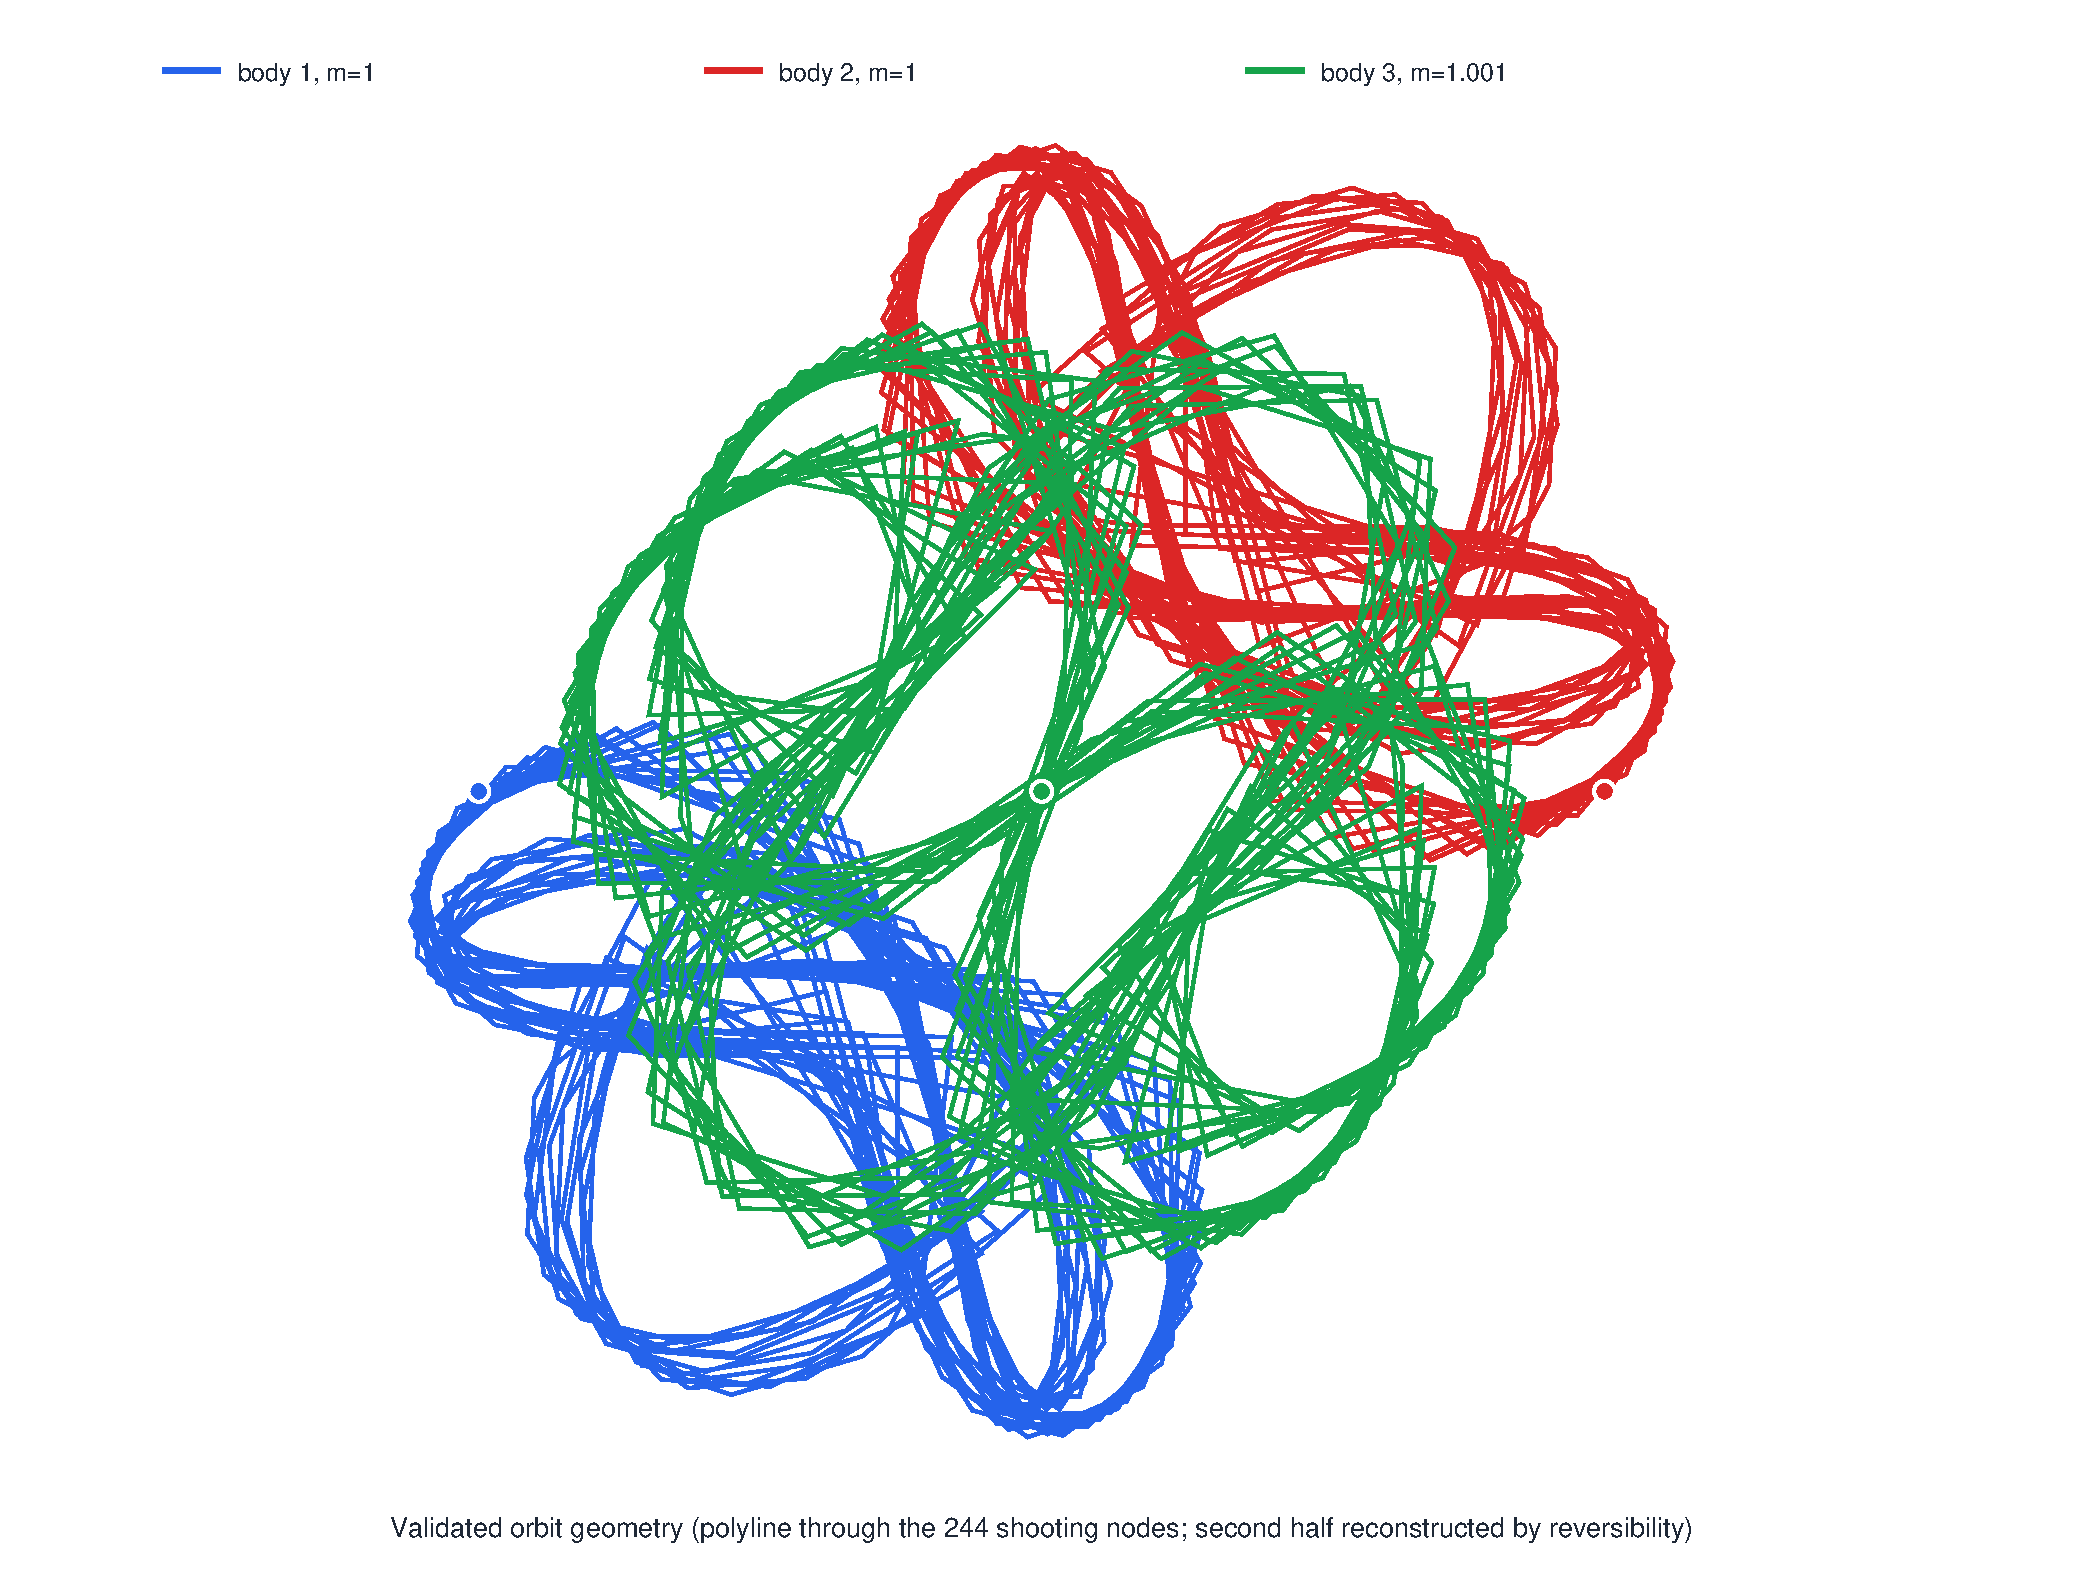
\includegraphics[width=0.78\linewidth]{orbit_geometry.pdf}
  \caption{Numerical geometry over one displayed period. The two unit masses are bodies 1 and 2; body 3 has mass $1001/1000$.}
  \label{fig:orbit}
\end{figure}

The numerical energy is approximately $-1.3818502425450523$ and the scale-invariant period $T|E|^{3/2}$ is approximately $314.993513098724$. Event-refined numerical integration gives sampled minimum distance $0.0610408983$ and the syzygy sequence
\begin{equation}
  (2132123123123213)^{13}, \label{eq:word}
\end{equation}
which identifies the geometry as a Moth-I$^{13}$ topological-power satellite in the standard equal-outer-mass labeling \cite{suvakov-dmitrasinovic-2013,hudomal-2018}.

Because \eqref{eq:word} is a proper power, topology does not prove dynamical primitivity. A derivative-refined scan of the identity-return norm on $0<t<T$ found the smallest earlier stationary return to be approximately $1.1622\times10^{-2}$, while the endpoint residual of an independent ordinary integration was $9.9\times10^{-10}$. At the twelve checkpoints $kT/13$, all identity-return distances exceeded $1.6729\times10^{-2}$. These are strong numerical indicators that the orbit is not a 13-fold traversal, but they are not a global interval lower bound. Theorem~\ref{thm:main} therefore proves a $T$-periodic orbit, not that $T$ is its minimal period.

\section{Finite catalog audit}

The candidate was compared modulo translation, rotation and reflection, time shift and reversal, Newtonian similarity scaling, and simultaneous relabeling of positions, velocities, and masses. Topological words were reduced modulo the corresponding cyclic, reversal, and relabeling equivalences before coordinate-level comparison.

The principal unequal-mass survey of Li, Jing, and Liao reports 1,349 families at the sampled third masses $0.5,0.75,2,4,5,8,10$, not at $1001/1000$ \cite{li-jing-liao-2018}. The later one-family supplement does contain the exact mass triple, but every member continues the one-copy word \texttt{bABabaBAba}; its row at $(1,1.001,1)$ has listed period about $7.54087$ and is topologically distinct from Moth-I$^{13}$ \cite{li-li-liao-2021}. Large Sofia supplements concern the equal-mass problem and therefore cannot contain the exact unequal-mass orbit considered here \cite{hristov-2025}. Searches of the other documented absolute and relative periodic families examined in the accompanying audit found no equivalent record.

This establishes a finite catalog nonmatch, not an exhaustive priority theorem. The defensible novelty statement is:
\begin{quote}
  Theorem~\ref{thm:main} validates an apparently uncatalogued unequal-mass realization of the known Moth-I$^{13}$ class at masses $(1,1,1001/1000)$.
\end{quote}
Neither the Moth-I topology nor the equal-mass seed is claimed as new. Unpublished computations, inaccessible data, or a future catalog may contain an equivalent orbit.

\section{Reproducibility and proof boundary}

The public repository contains the exact center and radii, 244-node mesh, center and outer interval enclosures, source code, compiler flags, archived logs, and two verification routes. The quick route recompiles the checkers and verifies the archived enclosures; the full route regenerates all local integrations before assembling the final certificate. The release artifact is available at
\begin{center}
\url{https://github.com/Rexyysilent/three-body-moth13-cap/releases/tag/v1.0.0-rc1}.
\end{center}
The release ZIP has SHA-256 digest
\begin{center}
\texttt{a645abf8111b9ad8d0d70e766f4fffd6ca1550373d81b80146953698ff8cf619}.
\end{center}

The following claims are machine-certified: an exact zero of the shooting equations in the stated box; periodic closure by the analytic reversibility argument; local uniqueness in the box; and the global collision bound \eqref{eq:collision-bound}. The following are not claimed as interval-certified: minimal period, the complete syzygy itinerary, linear stability, a quantified mass interval for Corollary~\ref{cor:family}, or unconditional catalog novelty.

\paragraph{Authorship and computational assistance.}
Rexyysilent is the sole author and accepts responsibility for the claims, source, and presentation. OpenAI Codex using GPT-5.6 Sol provided substantial assistance with numerical-search orchestration, proof engineering, literature and catalog auditing, code review, and manuscript drafting. The AI system is acknowledged as a tool and contributor, not as an author.

\paragraph{Licensing.}
Code in the accompanying repository is licensed under Apache-2.0. Documentation, manuscript source, figures, logs, and data are licensed under CC BY 4.0 unless a file states otherwise.

\paragraph{Verification invitation.}
Independent reruns should report the commit, platform, compiler, dependency versions, command, stdout, stderr, wall time, and final certificate hash in the public verification issue:
\begin{center}
\url{https://github.com/Rexyysilent/three-body-moth13-cap/issues/1}.
\end{center}

\bibliographystyle{plain}
\bibliography{references}

\end{document}
